\section{Outline of the Construction}

\eat{Suppose that one has a system of linear equations
  $e_1=0,\ldots,e_m=0$ over Boolean variables $x_1,\ldots,x_n$. Using
  the machinery described in Section~\ref{section:Tensoring}
  (tensoring), one can produce a new system of linear equations, over
  new Boolean variables, that has a larger fraction of satisfiable
  equations. If we apply tensoring to a linear PCP, both the
  completeness error $\delta$ and one minus the soundness error $1-s$
  are raised to the power $k$. Thus, we follow the product operation
  with an operation that picks (in some pseudorandom way) $t\approx
  1/(1-\delta)^k$ equations and tests all of them (in fact, we will
  perform the linear analog of this product operation: the one that
  takes random linear combinations of $t$ equations: $\sum_i \alpha_i
  e_i = 0$).  This distinguishes between the case of having just
  $\delta$ unsatisfiable equations and the case of having $1-s$
  unsatisfiable equations. In other words, it preserves the low
  completeness error, and decreases back the soundness error.  Even
  when doing that, tensoring has several downsides:
\begin{enumerate}
\item\label{p:prod.size} The number of equations raises to the power
  $k$.
\item\label{p:prod.queries} Each equation depends on $k$ times as many
  variables.
\end{enumerate}
Item~\ref{p:prod.queries} can be fixed using PCP techniques for query
reduction. Item \ref{p:prod.size} is more challenging. There is a way
to fix item~\ref{p:prod.size} by derandomization, but it results in
non-linear equations.  In fact, the tensoring approach is exactly the
route taken by Khot and Ponnuswami~\cite{KP}, and is the reason for
their large blow-up. In this paper we find a way to preserve linearity
without incurring a large blow-up.

\subsection{Our Idea}}

We start with a construction of a binary linear PCP based on H\aa
stad's \textsc{Max-3Lin} construction~\cite{Has97}
(Section~\ref{section:basic}). Importantly, this PCP is an
``assignment tester'', a certain strengthening of PCP that is needed
later. We preserve this strong PCP property throughout the opertations
we perform on this PCP.  We perform tensoring to amplify the
completeness of the basic construction in
Section~\ref{section:complete} (getting a ``longer long code'').
Tensoring increases the number of satisfied equations, and so
decreases the completeness error, but increases the soundness
error. Hence, in Section~\ref{section:complete}, we follow tensoring
with a randomness-efficient sequential repetition that preserves
linearity and the low completeness.

This inner construction is then composed with an outer construction
with perfect completeness in Section~\ref{section:composition}. The
outer construction is not linear. However, since the inner
construction is based on the long code, the composed construction can
still be linear, just like H\aa stad constructs linear verifiers out
of non-linear verifiers in \cite{Has97}.

In the second phase of our construction
(ref. Section~\ref{section:sound}), we leverage the low completeness
error to boost the soundness to $1/{\cal O}(\log N)^\beta$ for some
$\beta >0$. Specifically, we use techniques from \cite{MR08} to
amplify the soundness while preserving the linearity of the
verifier. This yields a family of {\sf Label-cover} instances whose
constraints are linear projections. Note that the \cite{MR08}
transformation produces a PCP with the projection property (two
queries), even when starting with a PCP with many queries.

The applications for \textsc{Max-3Lin} and \textsc{Max-3Sat} are
presented in Section \ref{section:hardness}. The linearity of our
construction enables us to use Hadamard codes rather than Long
codes. To the best of our knowledge, Khot \cite{Khot01} was the first
to construct Hadamard based PCPs.

The construction described above is our ``simple construction'', and
it only yields logarithmically-small completeness error. We proceed to
a more complicated construction that yields polynomially-small
completeness error. This is needed for our hardness results for
\textsc{Min-3Lin-Deletion} and \textsc{Nearest-Codeword-Problem}, and
also to achieve optimal results for \textsc{Max-3Lin} and
\textsc{Max-3Sat} assuming Conjecture~\ref{c:soundness}.  For the
construction of PCPs with polynomially small completeness error we use
an iterative construction, performing tensoring and query
reduction. This is done in Section~\ref{section:Iterated}. The outline
of our construction is also presented in Figure~\ref{figure:layout}.

\begin{figure}[hp]
\centering
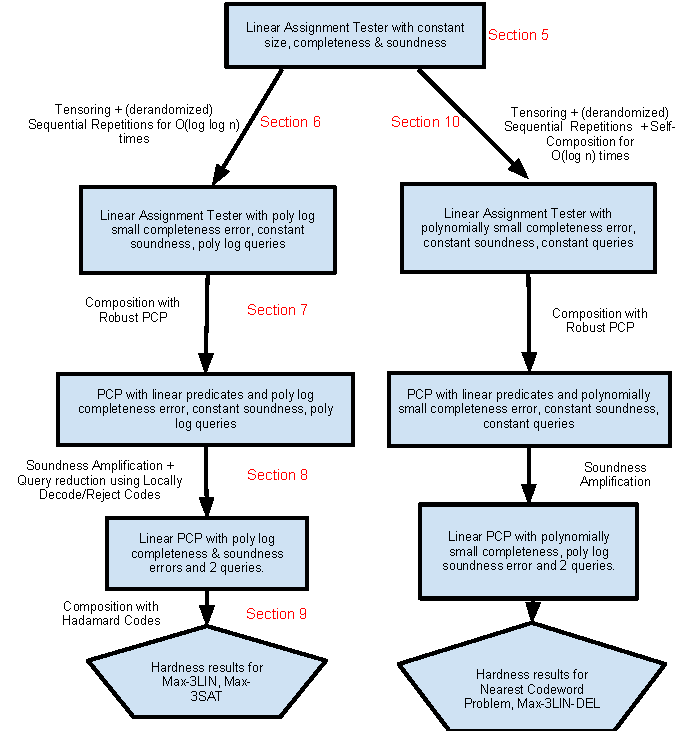
\includegraphics{Layout}
\caption{Layout of our Construction.}
\label{figure:layout}
\end{figure}

\newpage
%{\huge{Appendix}}

\section{Assignment Testers} \label{section:basic} In this section, we
construct a PCP verifier with a linear tests. In what follows, we work
with assignment testers. The notion of assignment testers was
pioneered by \cite{DR,BGHSV,S99}. They are (also) sometimes referred
to as PCP of Proximity. A related notion was recently explored as
Locally Decode and Reject Codes (LDRC) \cite{MR08} (ref. Definition
\ref{def:LDRC}) and as {\sf dPCP} by \cite{DH}.  Informally, an
assignment tester not only needs to accept a correct proof almost
always, but reject a purported proof which is far from any valid
proof. Note that this is a stronger requirement to that of a PCP where
one aspires to verify only if there is a valid proof or not. We
restrict ourselves to {\em linear} assignment testers. These are
assignment testers where the verifier's predicate is a linear function
over its variables.

\begin{definition}[Assignment Tester] \label{AT} An $(1 - \rho,
  \delta)$-Assignment Tester is a reduction whose input is a Boolean
  constraint $\psi$ over a set of Boolean variables $X$. The output of
  the reduction is a system of constraints $\Psi$ over variables $X$
  and auxiliary variables $Y$ such that for every assignment $\pi: X
  \rightarrow \{0,1\}$,
\begin{itemize}
\item {\sf Completeness:} If $\pi$ satisfies $\psi$ then there exists
  an assignment $\tilde{\pi} : Y \rightarrow \{0,1\}$ such that $\pi
  \cup \tilde{\pi}$ satisfies at least $1 - \rho$ fraction of
  the constraints in $\Psi$.
\item {\sf Soundness:} For every $\delta' < \delta$, if $\pi$ is
  $\delta'$-far from a satisfying assignment for $\psi$, then for
  every assignment $\tilde{\pi}: Y \rightarrow \{0,1\}$, at least
  $\Omega(\delta')$ fraction of the constraints in $\Psi$ reject $\pi \cup
  \tilde{\pi}$.
\end{itemize}
\end{definition}

From now on, it will be useful to use the set $\{+1 , -1\} = \{\pm
1\}$ instead of $\{0,1\}$. We use the following map $b \mapsto (-1)^b$
(that is, $0 \mapsto 1$ and $1 \mapsto -1$). Also note that this maps
the addition in $GF(2)$ into multiplication operation over
$\mathbb{R}$.


\paragraph{Standard Definitions.} We identify the {\em long code} of
${\bf x} \in \{\pm 1\}^s$ by $\LC$({\bf x}) $= \{ f({\bf x}) | f :
\{\pm 1\}^s \rightarrow \{\pm 1\} \}$. Informally, we evaluate {\bf x}
on every Boolean function on $s$ bits. Notice that every Boolean
function on $s$ bits may be represented by its truth table. In other
words, by specifying its evaluation on all the $2^s$
inputs. Alternatively, any string of length $2^s$ may be interpreted
as a Boolean function on $s$ bits. We denote $2^s$ by $n$. Since,
there are $2^{n}$ Boolean functions on $s$ bits, $\LC({\bf x})$ is a
string on length $2^{n}$. We use the letters $f, g$ to denote Boolean
functions. It is easy to check that given a table $A$, $ A \equiv
\LC({\bf x} : \{ \pm 1\}^s \rightarrow {\pm 1}$, $A(f) A(g) =
A(fg)$. That is, $A$ is closed under multiplication.

For $\alpha \subset [n]$, define
\[
          \chi_\alpha : \{\pm 1\}^n \rightarrow \{\pm 1\},  \chi_\alpha(f) \triangleq \prod_{i\in \alpha}f(i)
\]

It is easy to check that the characters $\{\chi_\alpha\}_{\alpha
  \subseteq [n]}$ form an orthonormal basis for the space of functions
$\{A : \{\pm 1\}^n \rightarrow \mathbb{R}\}$, where inner product is
defined by $\langle A, B \rangle = \mathbb{E}_f[A(f) B(f)] =
2^{-n}\sum_fA(f)B(f)$. It follows that any function $A: \{\pm 1\}^n
\rightarrow \{\pm 1\}$ can be written as $A = \sum_\alpha
\hat{A}_\alpha \cdot \chi_\alpha$, where $\hat{A}_\alpha =\langle
A,\chi_\alpha \rangle$.

\paragraph{The Long Code Test.}\label{LC} Let $A : \{ \pm 1\}^n \rightarrow \{\pm 1\}$. 
We intend to test if $A : \{\pm 1\}^n \rightarrow \{\pm 1\}$ is in
fact the legal encoding of a value $i \in [s]$. In other words, if
$A(f) = f(i)$ for all $f \in [2^n]$.

Fix a parameter $\rho \in [0,1]$. The test picks two uniformly random
vectors $f,g \in \{\pm\}^n$ and then ${h} \in \{\pm\}^n$ according to the
following distribution: for every coordinate $i \in [n]$, with
probability $1 - \rho$ we choose $h_i = 1$ and $h_i = -1$ otherwise.
It is useful to imagine ${h}$ as a noise vector. The test accepts iff
$A({f}) A({g}) = A({fgh})$.\eat{ In other words, iff $h_w = 1$, which
  happens with probability $1 - \rho$. It follows from the
  construction that the test accepts any valid long code encoding with
  probability $1 - \rho$. We now state a certain converse of that,
  which was establised by H{\aa}stad's lemma \cite{Has97}.
\begin{lemma}[H{\aa}stad's lemma \cite{Has97}]
  If the test accepts $A$ with probability $1/2 + \delta$, then
  $\sum_\alpha \hat{A}^3_\alpha \cdot (1 - 2\rho)^{|\alpha|} \ge
  2\alpha$.
\end{lemma}

\begin{lemma}[Corollary 22.25 in \cite{AB}]
  For every $\delta, \epsilon > 0$, if $A$ passes the long code test
  with probability with $1/2 + \delta$, then for $k =
  \frac{1}{2\rho}\log\frac{1}{\epsilon}$, there exists $\alpha$ with
  $|\alpha| \le k$ such that $\hat{A}_\alpha \ge 2\delta - \epsilon$.
\end{lemma}
}
\newcommand{\E}[2]{{\mathbb{E}}_{#1}\left[#2\right]}
%\newcommand{\expect}[2]{{\mathbb{E}}_{#1}\left[#2\right]}

\begin{lemma}[Tester Lemma]\label{longcode}
  For every $\delta > 0$, table $A$ which is $\delta$-far from any
  valid long code encoding is rejected with probability at least
  $\Omega(\delta)$.
\end{lemma}
\noindent {\em Proof.}  Assume that $A$ passes the test with
probability $1 - \delta$, then $\E{}{A(f)A(g)A(fgh)} = 1 -
2\cdot\delta$. Replacing $A$ by its Fourier expansion, we have

\begin{align*}
  1 - 2 \cdot \delta  &= \E{f,g,h}{\left(\sum_\alpha \hat{A}_\alpha\chi_\alpha(f) \right) \cdot \left(\sum_\beta \hat{A}_\beta\chi_\beta(g) \right) \cdot \left(\sum_\gamma \hat{A}_\gamma\chi_\gamma(fgh)\right)}\\
 &=\E{f,g,h}{\sum_{\alpha,\beta,\gamma}\hat{A}_\alpha\hat{A}_\beta\hat{A}_\gamma\chi_\alpha(f) \chi_\beta(g) \chi_\gamma(f) \chi_\gamma(g) \chi_{\gamma}(h)}\\
 &= \sum_{\alpha,\beta,\gamma}\hat{A}_\alpha \hat{A}_\beta \hat{A}_\gamma \E{f,g,h}{\chi_\alpha(f) \chi_{\beta}(g) \chi_{\gamma}(f) \chi_{\gamma}(g) \chi_{\gamma}(h)}
\end{align*}

\noindent Since the fourier basis are orthonormal, the expectation is $0$ unless $\alpha = \beta = \gamma$. Therefore,
\[
1 - 2\delta = \sum_\alpha \hat{A}_\alpha^3 \E{h}{\chi_\alpha(h)}\\
\]
\noindent Because $\E{h}{\chi_\alpha(h)} = \E{h}{\prod_{w \in
    \alpha}h_w} = (1 - 2\rho)^{|\alpha|}$, as each coordinate of $h$ is
chosen independently. Hence,
\begin{align*}
  1 - 2 \delta &= \sum_{\alpha} \hat{A}_\alpha^3 (1 - 2\rho)^{|\alpha|} \\
  &\le \sum_{\alpha} \hat{A}_\alpha^2 \cdot 1 \cdot (1 - 2\rho)^{|\alpha|} \ \ \ \ \  \ \  \because \hat{A}_\alpha \le 1\\
  &\le \sum_{|\alpha| =1} \hat{A}_\alpha^2 (1 - 2\rho) + \sum_{|\alpha| > 1} \hat{A}_\alpha^2 (1 - 2\rho)^{|\alpha|}, \ \ \  \ \hat{A}_\emptyset = 0 \ \ \mbox{due to folding}
%  &\le \sum_{|\alpha| =1} \hat{A}_\alpha^2 (1 - 2\rho) + \sum_{|\alpha| > 1} \hat{A}_\alpha^2 (1 - 2\rho)^{|\alpha|}  \\
 \end{align*}

 \noindent Since $A$ is assumed to have been folded, $\hat{A}_{\alpha}
 = 0$ if $|\alpha|$ is even. Hence, $(1 - 2\rho)^{|\alpha|} \le (1 -
 2\rho)^{3}$.  Therefore, the above expression can be written as follows.
\begin{align*}
  1 - 2\delta &\le \sum_{|\alpha| =1} \hat{A}_\alpha^2 (1 - 2\rho) + \sum_{|\alpha| > 1} \hat{A}_\alpha^2 (1 - 2\rho)^{3} \\
  & \le (1 -\Phi) (1 - 2\rho) + \Phi ( 1 - 2\rho)^{3} \ \ \ \  \ \ \
  \mbox{Let} \sum_{\alpha, |\alpha| > 1}\hat{A}^2_\alpha = \Phi\\
 1 - 2\delta &\le (1 - 2\rho) (1 - \Phi + \Phi (1 -2 \rho)^2) \\
{1 - 2\delta}/{1 - 2\rho} & \le (1  - \Phi (1 - (1 - 2\rho)^2)\\             
1 - 2(\delta - \rho) & \le 1 - \Phi (1 - (1 - 2\rho)^2)\\
\Phi & \le 2(\delta - \rho)/(4\rho - 4\rho^2)
\end{align*}
\noindent Since, $\rho$ is a fixed parameter, we have $\Phi = {\cal
  O}(\delta)$ At which point, we recall a result of Friedgut, Kalai
and Naor \cite{FKN} which (informally) states that if the fourier
coefficients are concentrated on the lowest two levels, then the
function is close to a constant function or a function that is
determined by a single coordinate.

\begin{theorem}[Theorem B.4, Page 41 in \cite{Dinur}]\label{FKN}
  There is a global constant $C'$ (independent of $n$) such that the
  following holds. Let $\Phi > 0$ and let $A : \{1, -1\}^n \rightarrow
  \{1, -1\}$ be a Boolean function for which $\sum_{\alpha, |\alpha|
    >1} |\hat{A}_\alpha|^2 < \Phi$. Then either $|\hat{A}_\emptyset|^2
  \ge 1 - C'\Phi$, or for some $i \in [n]$, $|\hat{A}_{\{i\}}|^2 = 1 -
  C'\Phi$.
\end{theorem}


\noindent Therefore, by folding, there must be some $i$ such that $\psi(i) = -1$
and $\chi_{i}$ is ${\cal O}(\Phi)$. Theorem \ref{FKN} also allows $-
\chi_i$ to be ${\cal O}(\Phi)$-close to $A$, but this causes the test
to fail with probability close to $1/4$, which is certainly
$\Omega(\delta)$. Hence, we showed that unless $A$ is $\delta$-close
to some $\chi_{i}$ for the value of $i$ that satisfies $\psi$, at
least $\Omega(\delta)$ of the tests must be
rejected. \qed \\






\eat{That is,
\begin{align*}
  \	   \Pr \left [A\ \mbox{passes}\ \right]  &\ge 1 - \delta \\
  & \implies   \hat{A}_k \ge 2 \cdot (1/2 -\delta ) - \epsilon \\
  &\implies  \exists \alpha \subset [n],  |\alpha|  \le k \  \mbox{s.t.}\  \chi_\alpha \  \mbox{is}\  \Omega(\delta')\mbox{-far}\ \mbox{from}\  A \\
 \end{align*}
 Note that $\chi_\alpha$ can be expressed as $\prod_{i \in \alpha}
 \chi_i$ and $|\alpha|$ is a constant.  Thus, any of the $\chi_i$'s
 agrees with $\chi_\alpha$ on at least $2^{-|\alpha|}$ fraction of the
 domain. Putting this in the context of agreement between $A$ and
 $\chi_i$: $\chi_i$ disagrees with $A$ on at least $1/2^{|\alpha|}
 \cdot \delta'$ fraction, which is essentially
 $\Omega(\delta)$. \qed\\}

  
 
\noindent We are now ready to present the assignment tester needed for
our construction. Let $\psi$ be a Boolean constraint over Boolean
variables $x_1, x_2 \ldots x_s$. We describe an algorithm whose input
is $\psi$ and whose output will be a system of linear equations
satisfying the requirements of Definition \ref{AT}. The tester seeks
as input a satisfying assignment $\sigma$ to $\psi$ and the
$\LC(\sigma)$, the long code of $\sigma$. One may imagine $\LC(\sigma)$
as the set of auxilary variables used by the tester. \\

 
\noindent Also, as done in \cite{BGS}, we fold the long code tables
over true and the respective constraint $\psi$. This means that
whenever the test needs to read $A[f]$, it reads $A[\psi \wedge f]$
instead. In addition, we fold over true which means for every pair $f$
and $-f$, we let $A$ specify only one and access the other via the
identity $A[f] = - A[f]$. In short, we assume that $A[f] = A[f \wedge
\psi]$ and $A[f] =- A[-f]$ for all $f$. It is well known that after
folding $\hat{A}_\alpha = 0$ whenever $|\alpha|$ is even or there
exists an $i$ in $\alpha$ for which $\psi(i) = 1$ (recall that $1$
corresponds to false). An interested reader may refer to Lemma 22.27
on page 482 of \cite{AB}. We elaborate on the latter. Set $f' = f +
e_i$, where $i$ is an index such that $\psi(i) = 1$. Now,
$\chi_\alpha(f) = - \chi_\alpha(f')$ but $A[f] = A[f']$. We now
describe the two kinds of constraints we place over these
variables. Say, the tester gets two tables $\sigma$ and $A$ as input.

\begin{enumerate}
\item {\sf Long Code Constraints:} The first set of constraints aims
  at testing if $A$ is indeed a valid long code encoding. It includes
  $3$ variable constraints derived from the {\em long code} test
  specified earlier. Specifically, we shall fix $\rho$ to be a
  non-zero constant and have one constraint per each coin toss of the
  long code test.

\item {\sf Consistency Constraints:} The second set of constraints
  include the following: For each choice of $i \in [s]$ and $f$
  place a constraint that is satisfied iff $\sigma(x_i) = A(f) \oplus
  A(f \oplus e_i)$\footnote{$e_i$ is the vector of dimension $2^s$
    with a $-1$ in $i$-th index and $1$ elsewhere.}. For the ease of
  argument, assume that are an equal number of constraints of each
  type\footnote{This can be easily achieved by placing multiple copies
    of the constraint of each type with appropiate multiplicity.}.
\end{enumerate}

\begin{lemma}[Assignment Tester] \label{Tester} For any $\rho, \delta
  > 0$, the constraint system constructed above is a $(1- \rho,
  \delta)$-assignment tester for any Boolean function $\psi : [s]
  \rightarrow \{0,1\}$. Moreover, the assignment tester is a linear
  function on its input.
\end{lemma}
\noindent {\em Proof.} Linearity of the constraints follows from
construction. We now analyze the parameters of the tester below
parameter by parameter.

\begin{itemize}
\item {\em Completeness:} We set the probability of generating the
  noise vector {$h$} in the long code test to $1 - \rho$. Now, for any
  good assignment that satisfies the constraint $\psi$, the second set
  of constraints are always satisfied. The only case where we reject a
  good proof is during the long code test and this happens with
  probability at most $\rho$.

\item {\em Soundness:} Say, the tester gets $\sigma$ and $\pi$ as
  input and $\sigma$ is $\delta$-far from a satisfying assignment of
  $\psi$, we shall show that the assignment tester rejects with
  probability at least $\Omega(\delta)$. {\em w.l.o.g}, we consider
  the following cases. (1) $\pi$ is $\delta$-far from any long code
  encoding. (2) $\pi$ is not $\delta$-far from a valid long code
  encoding. \\

  \noindent In the former, it follows from Lemma \ref{longcode} that
  if $\pi$ is $\delta$-far from a valid long code table is rejected
  with probability greater than $\Omega(\delta)$ and by our
  construction these constraints constitute at least
  $\Omega(\delta)$-fraction of the total constraints. Thus, we reject
  any $\pi$ that is $\delta$-far from a valid long code encoding with
  probability at least $\Omega(\delta)$.


  In the latter, since $\pi$ was folded across $\psi$, we may assume
  that $\pi$ encodes a satisfying assignment to $\psi$. Say $\pi$
  encoded a satisfying assignment ${\sigma'}$. Since, $\sigma$ is
  $\delta$-far from a satisfying assignment, it must be that $\sigma$
  is $\delta$-far from ${\sigma'}$. Hence, $Pr_i[\sigma(x_i) \ne
  \sigma'(x_i)] \ge \delta$. Since, $\pi$ is not $\delta$-far from a
  valid long code encoding, we also have that
\begin{align*}
  \Pr_{f \in [n]} \left[ \pi(f) \oplus \pi(f +e_i) = f(\sigma') \oplus (f \oplus e_i)(\sigma') \right] & \ge \Pr [\pi(f) = f(\sigma') \ \ \mbox{and} \ \ \pi(f \oplus e_i) = (f \oplus e_i)(\sigma') ] \\
 &\ge 1 - 2\delta
\end{align*}
This fails whenever $\sigma(x_i) \ne \sigma'(x_i)$, then $f(\sigma')
\oplus (f \oplus e_i)(\sigma') = \sigma'(x_i) \ne \sigma(x_i)$. And
this is at least $\delta (1 - 2\delta) = \Omega(\delta)$. \\

\noindent Hence, in either case we would have rejected $\sigma \circ
\pi$ with probability at least $\Omega(\delta)$. Because, there are an
equal number of constraints of each type, we reject an invalid proof
$\pi$ with probability at least $\Omega(\delta)$.

\item {\em Query Size:} The tester picks at random a long code
  constraint or a consistency constraint and verifies it. In either
  case, it makes $3$ queries.

\item {\em Randomness:} The tester uses $2 \cdot s$ bits of
  randomness. \qed
\end{itemize}



We denote the {\sf size} of a linear tester by the $n$ and it refers
to the quantity $q \cdot m$, where $q$ is the number of queries made
by the tester and $m$ is the total number of equations in the
tester. Linear assignment testers cannot have perfect completeness.
For otherwise, one may use guassian elimination to figure out the if
there is an assignment that satisfies all the linear constraints and
reject if there isn't one. Hence, any linear tester is forced to have
a non-zero completeness error. Also, the soundness is always less than
$1/2$ as a random assignment satisfies at least $1/2$ of the equations
in $\eL$ in an expected sense (follows from the fact that the
equations are over ${GF}(2)$). As highlighted earlier, having low
completeness error becomes handy in several scenarios. We now
highlight on how we intend to use the tools we developed in the
previous section to achieve completeness amplification.


\section{Completeness Amplification}  \label{section:complete}

In this section, we employ tensoring to amplify the completeness of
the assignment tester we have built in Section \ref{section:basic}.
In what follows, we start with notations and a few observations that
will be useful to us in amplifying the completeness of the assignment
tester.\eat{ Let $\eL \equiv {\bf Ax} + {\bf y} = {\bf 0}$ denote the
  linear assignment tester given to us by Lemma \ref{Tester}. We now
  show that the d($\A$), d($\A$) $\equiv \min_{{\bf x} \ne {\bf 0}}
  {\bf Ax}$, is non-zero.

\begin{proposition}\label{longcodeisbest}
  Let $\eL \equiv {\bf Ax} + {\bf y} = {\bf 0}$ be the assignment
  tester obtained via Lemma \ref{Tester}. Then, for every ${\bf x_1}$
  and ${\bf x_2}$, ${\bf x_1} \ne {\bf x_2}$, the Hamming weight of
  ${\bf A} \cdot ({\bf x_1} + {\bf x_2})$ is a non-zero quantity. In
  other words, d($\A$) $> 0$.
\end{proposition}
\noindent {\em Proof.} To establish this, we consider the long code
constraints. Observe that the constants in the long code constraints
arise from the noise vector {h}. Thus, modulo the noise vector the
long code constraints are over auxilary variables $\pi$ of the tester
and are the following: $\Pi$ = $\pi(i) + \pi(j) + \pi(i + j) \ \forall
\ i,j \in |\pi|$. Now, since ${\bf x_1} \ne {\bf x_2}$, they either
differ on exactly $0 < k \le |\pi|$ coordinates. ${\bf x_1}$ and ${\bf
  x_2}$ evaluate different on every equation in $\Pi$. In the latter,
say they disagree on $\pi({\bf 0})$, then they evaluate differently on
$\pi(\alpha) + \pi({\bf 0}) + \pi(\alpha + {\bf 0})$. If however they
agree on $\pi({\bf 0})$, then either they disagree only one coordinate
$\beta$ or on more than one coordinates. In the former, ${\bf x_1}$
and ${\bf x_2}$ disagree on $\pi(\beta) + \pi(\alpha) + \pi(\alpha +
\beta)$. \qed }

\begin{definition} Let ${\cal T}$ denote the assignment tester
  obtained via Lemma \ref{Tester} and $\psi : [s] \rightarrow \{0,1\}$
  denote the Boolean predicate being tested. For any proof $\Psi$
  provided to ${\cal T}$, we denote by $\Pi_\psi$ the assignment
  induced by $\Pi$ on the variables of $\psi$. Also, we denote by
  $\psi(\Pi_\psi)$ the evaluation of $\psi$ on $\Pi_\psi$. 
\end{definition}

\begin{observation} \label{invariant} For any given proof $\Pi$ to
  assignment tester ${\cal T}$ to verify the satisfiability of $\psi$,
  $\Pi^{\otimes 2}_\psi$ is exactly same as $\Pi_\psi$. More
  importantly, the distance of $\Pi_\psi$ to a satisfying assignment
  of $\psi$ remains uneffected by tensoring. Moreover, the converse
  also holds. That is, for any purported proof $\Pi$ to a tensored
  system and its the diagonal entries, denoted by $\pi$, $\pi_\psi$ is
  same as $\Pi_\psi$.
\end{observation}
\noindent {\em Proof Sketch.} Since, we are working with $GF(2)$, it
follows from the defintion of tensoring that the diagonal entries
$\{x_{ii}\}$ of $\Pi^{\otimes 2}$ preserve $\Pi$. Thus, $\Pi_\psi$ and
$\Pi^{\otimes 2}_\psi$ are exaclty the same. The converse follows from
the fact that we extract (decode) the assignment $\pi$ from $\Pi$ by
reading
its diagonal entries. \qed\\


In fact, both directions of the aforementioned observation can be
extended to any $\Pi^{\otimes k}$, $\Pi^{\otimes j}, \ 0 < j \le
k$. We are now ready to amplify the completeness of the basic
assignment tester we have constructed in Lemma \ref{Tester}.

\begin{lemma}[Tensored Assignment Tester] \label{tensortester} For
  every $\rho, \delta > 0$, there is a $(1 - \rho^2,
  \delta^2)$-assignment tester for any Boolean function $\psi : [s]
  \rightarrow \{0,1\}$. Moreover, the predicate of the assignment
  tester is linear.
\end{lemma}
\noindent {\em Proof.} We invoke Lemma \ref{Tester} to construct an
$(1 - \rho, \delta)$-assginment tester ${\cal T}$. The tests performed
by our new $(1 - \rho^2, \delta^2)$-assginment tester, denoted by
${\cal T}^{\otimes 2}$, will be tensored tests of ${\cal T}$. In other
words, if the tests of ${\cal T}$ are $\eL$, then the tests of ${\cal
  T}^{\otimes 2}$ are linear equations in $\eL^{\otimes 2}$
(ref. Definition \ref{Tensoring}). Let $\Pi$ denote proof required by
${\cal T}$. The proof to $(1 - \rho^2, \delta^2)$-assginment tester
${\cal T}^{\otimes 2}$ will be ${\Pi}^{\otimes 2}$. Thus, the new
proof format will be $(\sigma \circ \pi)^{\otimes 2}$ and the
variables of $\psi$ will be $\{ \sigma_{ii}\}$ and the rest will be
auxilary variables of ${\cal T}^{\otimes 2}$. We shall now analyze the
parameters of ${\cal T}^{\otimes 2}$.
\begin{itemize}
\item {\em Completeness:} In the good case, if there is a proof
  $\sigma \circ \pi$ which ${\cal T}$ accepts with probability at
  least $1 - \rho$. We invoke Proposition \ref{basic} to conclude that
  the probability that ${\cal T}^{\otimes 2}$ accepts $\left(\sigma
    \circ \pi\right)^{\otimes 2}$ is at least $1 -$UNSAT($\eL, \sigma
  \circ \pi$)$^2$, which is $1 - \rho^2$.

\item {\em Soundness:} We shall establish that for any purported proof
  $\Pi$ to ${\cal T}^{\otimes 2}$, if $\Pi_\psi$ is $\delta^2$-far
  from a satisfying assignment to $\psi$, then ${\cal T}^{\otimes 2}$
  rejects with probability at least $\Omega(\delta^2)$.  In order to
  establish this, we deal with the contrapositive of the claim.  Say,
  if $\Pi$ is accepted with probabilty $1 - \delta^2$, we shall show
  that $\Pi_\psi$ is not $\Omega(\delta^2)$-far to a satisfying
  assignment of $\psi$.

  Say, $\Pi$ is accepted with probability at least $1 - \delta'$, we
  can use Lemma \ref{converse} to infer that the diagonal vector of
  ${\Pi}$ gives us a proof which ${\cal T}$ accepts with probability
  at least $\alpha = 1 - \lfloor \frac{\delta'}{\delta}\rfloor$, where
  $\delta' < 1/16$. For the parameters that we have choosen, if
  $\delta' = \Theta(\delta^2)$ then $\alpha \simeq 1 -
  \Omega(\delta)$. In other words, if $\Pi$ has an acceptance
  probability of $1 - \delta^2$, then we can decode a proof $\pi$,
  which ${\cal T}$ would accept with probability $1 -
  \Theta(\delta)$. And from Lemma \ref{Tester}, we know that if ${\cal
    T}$ accepts $\pi$ with probabilty $1 - \Theta(\delta)$, then
  $\pi_\psi$ isn't $\Omega(\delta)$-far from a satisfying assignment
  of $\psi$.

  But, from Observation \ref{invariant} we can infer that $\Pi_\psi$
  is exactly same as $\pi_\psi$. Thus, if $\pi_\psi$ is not
  $\delta$-far from a satisfying assignment of $\psi$, so is
  $\Pi_\psi$. Also, by hypothesis, ${\cal T}^{\otimes 2}$ accepts
  $\Pi$ with probability $1 - \Theta(\delta^2)$. Hence, we can
  conclude that for every $\Pi$, if $\Pi$ is accepted with probability
  at least $1 - \delta^2$, then $\Pi_\psi$ is not $\Omega(\delta)$-far
  from a satisfying assignment. Since $\delta^2 < \delta$, it follows
  that if $\Pi_\psi$ is $\delta$-far from a string, it is
  $\delta^2$-far. Therefore, the soundness of ${\cal T}^{\otimes 2}$
  holds.
\item {\em Query size:} ${\cal T}^{\otimes 2}$ needs to make as many
  queries as the number of variables in an equation of $\eL^{\otimes
    2}$. And this happens to be $\q^2$, where $\q$ is query size of ${\cal T}$.

\item {\em Randomness:} The randomness used by ${\cal T}^{\otimes 2}$
  is $\log \eL^{\otimes 2}$, which is $2 \cdot \log \eL$. In general,
  if we blow up the randomness by a factor of $k$ whenever we tensor
  an assignment tester $k$ times.\qed
\end{itemize}


\noindent Notice that the above transformation preserves the linearity
of the tester. The downside of tensoring is that while it enhances the
completeness, it also destroys the soundness. Ideally, we would like
to improve the acceptance probability of the verifier in the good case
and leave the acceptance probability in the bad case unperturbed. Thus
to improve the soundness of the tester after the tensoring operation,
we invariably resort to soundness amplification.

\subsection{Soundness Amplification Perserving Linearity}
Soundness amplification of a PCP can achieved via some kind of
repetition, either sequentially or in parallel. Repetition of a PCP
involves repeating the tests with independent randomness. For
instance, performing sequential repetition once would involve 
repeating the assignment tester on two independently drawn tests 
and accepting them iff both are satisfied. This transforms an $(1 - \rho,
\delta)$-assignment tester into an $(1 - 2 \cdot \rho ,2 \cdot
\delta)$-assignment tester. In general, performing sequential
repetition for $\vartheta$ times on $(1 - \rho , \delta)$-tester leaves us
with a $(1 - \vartheta \cdot \rho, \vartheta \cdot
\delta)$-tester. However, this operation does not preserve
linearity. 


Thus, we resort to a different kind of soundness amplification. We
pick ${\cal O}(1)$ tests of the assignment tester and then, adds all
possible linear combinations of these tests to the create a new
assignment tester. The idea is that even if one the ${\cal O}(1)$
 equations are not satisfied by some assignment, half of the linear
combinations of these equations will also not be satisfied by the
assignment. This also happens to preserve the linearity. However, to
keep the size of the output assignment tester instance small, we
pseudo-randomly generate only ${\cal O}(n)$ of the $n^{{\cal O}(1)}$
possible ways to pick ${\cal O}(1)$ tests from $n$ tests.

Given a $(1 - \rho^2, \delta^2)$-assignment tester as an input, we
wish to produce an $(1 - \rho^2, \delta)$-assignment tester as the
output. We achieve this via randoms walks on expanders. We aim to
achieve the following by taking a random walk on a expander: the
probablilty of visiting a subset containing a certain fraction
($\delta^2$ in our case) of the vertices is at least $2 \cdot
\delta$. And since, at least half of the linear combinations having an
unsatisfied equation also remain unsatisfied, we would end up with our
cherished objective of amplifying the soundness to $\delta$.

We begin by defining a {\em walk of length l} in a graph $G = (V,E)$
is a sequence $v_0, \ldots v_l$ of vertices of $G$, where for $1 \le i
\le l$, $v_{i-1}v_i$ is an edge in $G$. By a simple calculation, the
total number of walks of length $l$ in any $d$-regular graph is
exactly $|V|\cdot d^l$. Suppose there is a subset $C$ of $V$, we wish
to bound the number of walks that do not contain a vertex from $C$. If
$G$ happens to be disconnected, it may happen that a constant fraction
of them avoid $C$. However, Ajtai, Koml\'{o}s and Szemr\'{e}di
\cite{AKS87} showed that if all the eigenvalues of $G$, with the
exception of the largest, are small, then there are far fewer of walks
avoiding $C$. We now state their result.

\begin{theorem} \label{walks} Let $G = (V,E)$ be a $d$-regular graph
  on $n$ vertices, and suppose that each of its eigenvalues but the
  first one is at most $\lambda$. Let $C$ be a set of $cn$ vertices of
  $G$. Then, for every $l$, the number of walks of length $l$ in $G$
  that avoid $C$ does not exceed $(1 - c)\cdot n \cdot ((1 - c) \cdot
  d + c \cdot \lambda)^l$.
\end{theorem}

Now, a {\em randomly chosen walk} of length $l$ in $G$ chosen
according to a uniform distribution among all walks of that length.
If $G$ is regular, then such a walk can be chosen by choosing its
starting point $v_0$ uniformly at random and then picking the next
vertex of the walk among the $d$ neighbours of $v_0$ uniformly at
random. We are now ready to state a Corollary of Lemma \ref{walks}
which will be very useful for us.

\begin{corollary}\label{randomwalks}
  Let $G = (V,E), d, n, \lambda, C$ and $c$ be as in Theorem
  \ref{walks} and suppose 
\[
(1 - c)\cdot d + c \cdot \lambda \ \le \ \frac{d}{\sqrt{2}}
\]
Then, for every $l$, the probability that a randomly chosen walk of
length $l$ in $G$ avoids $C$ is at most $2^{{-l}/{2}}$.
\end{corollary}

\eat{In this work, we make use of a samplers based approach. Samplers
  are pseudo-random objects that are extremely useful in simulating a
  random walk or drawing random samples. In what follows, we denote
  the neighbours of a vertex $u$ in a graph by $\Gamma(u)$.

\begin{definition}[Samplers]
  A bipartite graph $H = (A,B,E)$ is said to be an $(\epsilon,
  \gamma)$-sampler if for every subset $S \subseteq A$,
\[
  \Pr_{b \in B}\left[ \frac{|\Gamma(b) \cap S|}{|\Gamma(b)|} > \frac{|S|}{|A|} + \epsilon \right] \le \gamma
\]
\end{definition}

In other words, neighbourhoods of most vertices $b$ behave like a
random sample of $A$, in the sense that that their density within any
fixed $S$ is close to what is expected.  The following article
\cite{Sample} by Oded Goldreich is an excellent exposition on
samplers, their constructions and applications.

\begin{theorem}\cite{Sample}\label{sample} There exists a polynomial 
  time algorithm that, given an integer $n$ and a parameter $\epsilon
  > 0$, outputs an $(\epsilon, \gamma)$-sampler with $|A| = |B| = n$
  and the right degree $4/\epsilon^4$. Moreover, the randomness used
  by the algorithm is bounded by $\log n + {\cal O}(\log 1/\epsilon )
  + {\cal O}(\log  1/\gamma)$.
\end{theorem}
}
\begin{lemma}[Soundness Amplification] \label{boosting} There is
  universal constant $\vartheta$, such that every $(1 - \rho^2,
  \delta^2)$-assignment tester for a Boolean predicate $\psi$ over
  variable set $\sigma$ can be amplified to a $(1 - \vartheta \cdot
  \rho^2, {\delta})$-assginment tester. Moreover, the new tester still
  has a linear predicate.
\end{lemma}
\noindent {\em Proof.} Let us denote the $( 1 - \vartheta \cdot
\rho^2), \delta^2)$-assignment tester by $V$ and the tests performed
by $V$ with $\eL$. Our approach will be to design a new assignment
tester $V'$ whose tests are the sum of $\vartheta$ tests of the old
verifier $V$. We construct a graph $G$ in which the vertices are the
tests of $V$. Let $\phi_i$ denote the equation (constraint) at vertex
$v_i$. We then pick a (test) vertex $v_1$ uniformly at random. We then
take a random walk of length $\vartheta$ starting at $v_1$. The new
tests will be the sum of tests at each of these vertices. Thus, $\eL'
= \{ \phi_1 \oplus \phi_2 \ldots \oplus \phi_\vartheta : \phi_i \in
\eL\}$. We fix $\vartheta$ to be the length of random that one must
take on an expander so that the probability we hit a $\delta^2$
fraction of the tests is at least $2 \cdot \delta$. It follows from
Corollary \ref{randomwalks} that for an appropiate choice of expander
and some constant $\vartheta$ less than $5$ it holds that the
probability we hit a $\delta^2$ fraction of the vertices is at least
$2 \cdot \delta$. Note that even though the tests of $V'$ are
different from $V$, both of them expect the same proof as in Lemma
\ref{Tester}. We now establish that $V'$ is in fact a $(1 - \vartheta
\cdot \rho^2, {\delta})$-assignment tester.
\begin{itemize}
\item {\em Completeness:} In the good case, $V$ reject a valid proof
  with probability at least $\rho^2$. Now by basic probability, the
  probability that $V'$ accepts a valid proof it is at most $(1 - \rho^2)^\vartheta$, 
  which is bounded from below by $(1 - \vartheta \cdot \rho^2)$.
 
\item {\em Soundness:} Say, we are given an assignment tester $V$ that
  rejects any proof $\Pi$ if $\Pi_\psi$ (projection of $\Pi$
  on the variable set $\sigma$) is $\delta$-far from a satisfying
  assignment of $\psi$, it is rejected with probability at least
  $\Omega(\delta^2)$. The claim we make is that the assignment tester
  $V'$ will get reject any $\Pi$ such that $\Pi_\psi$ is $\delta$-far
  from a satisfying assignment to $\psi$ with probabilty at least
  $\Omega({\delta})$. Consider the scenario that $V$ rejects a proof
  with probability $\delta^2$. It follows from our parameters 
  that probability the random walk hits the bad set is
  at least $2 \cdot \delta$ and at least half of these tests fail over
  the choice of our random walk. Thus, the probability the we accept
  an invalid proof is bounded from above by $1 - \delta$. In other
  words, if $V$ rejected an invalid proof with probability at least
  $\delta^2$, the new tester would reject it with probability at least
  $\delta$. The distance parameter of $\Pi_\psi$ is uneffected by this
  operation and hence, we inherit from Lemma \ref{Tester} and 
  \ref{tensortester} that if $\Pi_\psi$ was $\delta$-far from
  a satisfying assignment, it continues to be so.
 
\item {\em Query size:} The arity of the equations in $\eL'$ is $\vartheta
  \cdot q$, where $q$ is the arity of $V$.

\item {\em Randomness:} Since, we are choosing a test of $V$ uniformly
  at random and then taking a random walk of length $\vartheta$ on an
  expander $G$ with a constant degree, we would be needing $r_V +
  {\cal O}(\vartheta)$, where $r_V$ is the randomness used by $V$.\qed
\end{itemize}


\eat{
  \begin{lemma}[Derandomization Lemma] \label{derandomize} For every
    $\rho > 0, \delta < 1/4$, $\vartheta < \min(1/\rho,1/\delta)$ and
    $\vartheta$ sequential repetitons of every ($\rho,
    \delta$)-assignment tester can be achieved using only $r_v + {\cal
      O}(\vartheta)$ random bits.
\end{lemma}
\noindent{\em Proof.} Follows by invoking Theorem \ref{sample} to
construct a $(\epsilon, \gamma)$-sampler and use it instead of
sampling $\vartheta$ tests of verifier at random. Specifically, set $n
= 2^{r_v}$, $\gamma = 1- \vartheta \cdot \delta$, $\epsilon$ will be
fixed latter.  We now establish that this process actually simulates
sequential repetition in a randomness efficient way. During sequential
repetition, we wish to test independent samples of the verifier's
test. Consider the soundness case, here we would like to sample one of
the constraints that fail the verifier's test. Say, a set $S$ of the
tests fail. So, we would like to hit one of these tests. In a
sequential repetition, the probability that we hit this set is
$\vartheta \cdot \frac{|S|}{|A|}$.

We aim to achieve the aforementioned claims via a sampler. For a
sampler to have failed us, it must be that the vertex $b$ on the right
must have had all its neighbours in the complement (denote this set by
$\overline{S}$) of $S$ that we wanted to hit. And, the probability
that this would happen is
\begin{align*}
  \Pr_{b \in B}\left[ \frac{|\Gamma(b) \cap \overline{S}|}{|\Gamma(b)|} = 1 \right] 
  = \Pr_{b \in B}\left[ \frac{|\Gamma(b) \cap \overline{S}|}{|\Gamma(b)|} = 1 - \frac{|S|}{|A|} + \frac{|S|}{|A|} \right] 
  =  \Pr_{b \in B}\left[ \frac{|\Gamma(b) \cap \overline{S}|}{|\Gamma(b)|} =  \frac{|\overline{S}|}{|A|} +  \frac{|S|}{|A|} \right] 
%  =& \Pr_{b \in B}\left[ \frac{|\Gamma(b) \cap \overline{S}|}{|\Gamma(b)|} =  \frac{|\overline{S}|}{|A|} +  \frac{|S|}{|A|} \right] \\
  \end{align*}
We invoke Theorem \ref{sample} for $\epsilon \in (0, \frac{|S|}{|A|}]$.  
\begin{align*}
  \Pr_{b \in B}\left[ \frac{|\Gamma(b) \cap
      \overline{S}|}{|\Gamma(b)|} > \frac{|\overline{S}|}{|A|} +
    \epsilon \right] \le 1 - \vartheta \cdot \delta \implies \Pr_{b \in
    B}\left[ \frac{|\Gamma(b) \cap {S}|}{|\Gamma(b)|} > \epsilon
  \right] >  \vartheta \cdot \delta
\end{align*}

Hence, the completeness and soundness of this new assignment tester is
$\vartheta \cdot \rho$ and ${\vartheta} \cdot \delta$
respectively. This is essentially what we achieve with $\vartheta$
sequential repetitions as in Lemma \ref{boosting} but with a larger
query complexity $1/\epsilon^4$. If $\epsilon = \Theta(1/\vartheta)$,
then the query complexity happens to be ${\cal O}(\vartheta^4)$. The
bounds on randomness follows from Theorem \ref{sample}.
\qed\\
}
\begin{corollary}[Tensoring + Repetition]\label{iterate}
  For every $\rho > 0$ and $\delta < 1/4$, there is an absolute
  constant $\vartheta$, such that given an $(1 - \rho,
  \delta)$-assignment tester that uses $r_v$ random bits to make $\q$
  queries, one can construct an $(1 - {\cal O}\left(\rho^2\right) ,
  {\delta})$-assignment tester. The new assginment tester uses $2
  \cdot r_v + {\cal O}(\vartheta)$ random bits and makes ${\cal
    O}(\vartheta \cdot \q^2)$ queries. Moreover, our latest
  construction has a linear predicate.
\end{corollary}
\noindent {\em Proof.} We start with the assignment tester ${\cal T}$
given by Lemma \ref{Tester} that seeks a proof $\Pi = \sigma \circ
\pi$, where $\sigma$ are the variables of the Boolean predicate being
verified and $\pi$ is the auxilary variables introduced by the
assignment tester. Our new assignment tester ${\cal T}'$ is obtained
by invoking Lemma \ref{tensortester} and then followed by Lemma
\ref{boosting} on ${\cal T}$ with parameters $\delta = 16/100$,
$\vartheta = 5$ and $\rho = 1/\left(2 \cdot \vartheta\right)$ . The
proof required by ${\cal T}'$ will be $\Pi^{\otimes 2}$. We now argue
the completeness and soundness of the newly constructed assignment
tester.
\begin{itemize}
\item {\em Completeness:} In the good case, if we have a proof that
  the input assignment tester $T$ accepts with probability $1 - \rho$,
  we can use Proposition \ref{basic} to claim that after invoking
  Lemma \ref{tensortester} on $T$, we have a completeness of $1-
  \rho^2$. Now, after the application of Lemma \ref{boosting} it
  follows from our parameters that the completeness of $1 - {\cal
    O}(\rho^2)$.
\item {\em Soundness:} Say, the newly constructed assignment tester is
  given a purported proof $\Pi$ such that $\Pi_\psi$ (denotes the
  assignment induced on $\sigma$ by $\Pi$) is $\delta$-far from a
  satisfying assignment to $\psi$, we will need to establish that it
  is rejected with probability at least $\Omega(\delta)$. One
  important inference from Observation \ref{invariant} is that the
  neither tensoring nor soundness amplification change the assignment
  to $\sigma$ and hence, its distance to a satisfying assignment of
  $\psi$. Hence, if the input assignment tester has the soundness for
  $\delta < 1/4$, we can invoke the soundness arguments of Lemma
  \ref{tensortester} and \ref{boosting} to infer that soundness
  condition remains intact for $\delta < 1/4$. \qed
\end{itemize} 


\begin{lemma}[Completness Amplification Lemma]\label{Camplify}
  For every $\rho > 0$ and $\delta < 1/4$, given a $(1 - \rho,
  \delta)$-assignment tester with query complexity $\q = {\cal O}(1)$
  and size $2^{r_v}$, one can construct a $(1 - {\cal
    O}(\rho^k),\delta')$-assignment tester with query complexity $\q$,
  $\q = 1/\rho^{k'}$, in time polynomial in $2^{ k \cdot {\cal
      O}(r_v)}$. Also, the resulting assignment tester has a linear
  predicate.
\end{lemma}
\noindent{\em Proof.} Say we have a (1 - $\rho, \delta$)-assignment tester
that verifies a Boolean predicate $\psi$ using a proof over variables
of $\psi$ (call them $\sigma$) and auxilary variables $\pi$. The idea is to
let the tests of the $(1 - {\cal O}(\rho^k),\delta)$-assignment 
tester be the tests of lemma \ref{iterate} tensored with itself $k$ times. 
Our $(1 - {\cal O}(\rho^k),\delta)$-assignment 
tester uses the proof ($\sigma \circ \pi$)$^{\otimes k}$.

However, we would like to iteratively apply the output of Lemma
\ref{iterate} upon on itself. This makes it easier to apply the tools
that we have build thus far. The first observation we make is that the
after a $(1 - \rho, \delta)$-tester, of size $n$, under goes $r$
iterations of the tensoring followed by $\sigma$ rounds of sequential
repetition, the size of the resulting tester is
$n^{2^{2^{r-1}}}$. This can be verified once we observe that we are
squaring the size of the input instance in every iteration. By
invoking Corollary \ref{iterate}, we infer that the completeness error
is also squared in each iteration. Hence after $r$ iterations, the new
error parameter is $\rho^{2^{2^{r-1}}}$. However, the soundness of the
tester remains uneffected due to the amplification given by Lemma
\ref{boosting}. With this background, the Lemma follows by setting $ r
= \log \log k$. Notice that the proof required by this recursive
construction is same as that of the iterative assignment tester
constructed in previous paragraph.  The new proof will be $(\sigma
\circ \pi)^{\otimes k}$. Also, note that while the auxilary variables
blow up in every step, the variables of the Boolean predicate that we
are checking remain the same. The parameters are summarized in Table
\ref{roundup}.

\begin{table}
%\begin{table}
\centering
\begin{tabular}{|l|c|c|c|}
\hline
%\ & & \\
{\em Parameters}  &{ Tensoring} & {\parbox{0.9in}{Soundness\\ Amplification}} & \parbox{0.7in}{After $k$\\ Iterations}\\
	\hline
%\ &  & \\ 
        \hline
        {\tt Completeness} & $1 - \rho^2$ & 1 - ${\cal O}\left(\rho^2\right)$  & 1 - ${\cal O}(\rho^{k + 1})$ \\  
        {\tt Soundness} &   $\delta^2$ & $\delta$&  $\delta$ \\
        {\tt Queries} &   $q^2$ & $\vartheta\cdot q^2$ & $\vartheta^{\sqrt{k}+1} \cdot  q^{k} $ \\
        {\tt Alphabet}&    $\{0,1\}$ & $\{0,1\}$ & $\{0,1\}$ \\
        \hline
\end{tabular} %\caption{Parameters after one iteration} \label{1round}
  \caption{Parameters of a ($\rho, \delta$)-assignment tester after various operations.} \label{roundup}
\end{table}


\begin{itemize}
\item {\em Completeness:} It is by far the easier case to argue. Say,
  a $(1 - \rho, \delta)$-assignment tester is given to us that enables
  us to verify a Boolean predicate using a proof $\Pi$. Then by
  Corollary \ref{iterate}, we have a new assignment tester which has
  the square of the completeness error after a single iteration. It
  follows that after $\log \log k$ iterations, we end up with a
  completeness error of ${\rho^k}$.

\item {\em Soundness:} Say that the $(1 - {\cal
    O}(\rho^k),\delta)$-assignment tester is given access to a
  purported proof $\Pi$, we need to show that the if the proof
  $\Pi_{\psi}$ (denotes the assignment induced by $\Pi$ on the
  variables of $\psi$) is $\delta$-far to a satisfying proof of the
  Boolean predicate, the tester rejects with probability at least
  $\Omega(\delta)$. We show this property holds after each iteration
  and hence, the newly constructed assignment tester via this process
  always has the soundness condition.

  The approach is simple. We give a proof by induction on the number
  of iterations. The assignment tester produced after the first
  iterate is sound by Corollary \ref{iterate}. Assume that the
  assignment tester produced after $i$-th iterations is sound. We now
  show that the assignment tester produced after ($i+1$)-th iteration
  is also sound. By assumption, the assignment tester at the $i$-th
  level has the soundness property, it now follows from Corollary
  \ref{iterate} that the soundness holds even after $(i+1)$-th
  iteration.

\item {\em Queries:} We again invoke Corollary \ref{iterate} to
  conclude that the number of queries are first squared and then,
  multiplied by a factor of $\vartheta$ in every iteration. Since the
  basic tester of Lemma \ref{Tester} made $\q = {\cal O}$($1$)
  queries, after $\log \log k$ iterations we would have a query
  complexity of $\q^{k} \simeq 1/\rho^{k'}$.

\item {\em Randomness:} In every tensoring operation, we square the
  randomness (ref. Lemma \ref{tensortester}). Thus, the {\em
    randomness} of the tester after $r$ iterations is $k \cdot {\cal
    O}(r_v)$, where $r_v$ is the randomness used by the ($1 - \rho,
  \delta$)-tester of Lemma \ref{Tester}.

\item {\em Alphabet:} The alphabet of the tester obtained via Lemma
  \ref{Tester} has an alphabet $\{ 0,1\}$ and it remains unchanged
  during the application of Lemma \ref{iterate}. \qed
\end{itemize}




